\documentclass[12pt]{article} 
\usepackage{geometry} 
\geometry{a4paper} 
\linespread{1.1} % Line spacing


% FIGURES AND FLOATS
\usepackage{graphicx} % Required for including pictures
\usepackage{float} % Allows putting an [H] in \begin{figure} to specify the exact location of the figure
\usepackage{wrapfig} % Allows in-line images such as the example fish picture
\usepackage[font={small,it}]{caption}
\usepackage{subcaption}
\usepackage{epstopdf}
\graphicspath{{images/}}

% MATH
\usepackage{amssymb}
\usepackage{amsmath}
\usepackage{algorithm}
\usepackage[noend]{algpseudocode}

% OTHER
\usepackage[]{mcode}
\usepackage{enumerate}
\usepackage{xcolor}
%character
\usepackage{indentfirst} % 强制要求第一个段落也进行缩进
%段间距
\setlength{\parskip}{1ex plus 0.5ex minus 0.5ex}
%%%%%%%%%%%%%%%%%%%%%%%%%%%%%%%%%%%%%%%%%%%%%%%%%%%%%%%%%%%%
\usepackage{listings} 

%段首缩进
\setlength{\parindent}{2em} 

\definecolor{DeepPink}{RGB}{255, 20, 147}
\definecolor{LightSlateBlue}{RGB}{132, 112, 255}
\definecolor{ForestGreen}{RGB}{34, 139, 34}

\lstset{
  language=Matlab,  %代码语言使用的是matlab
  frame=shadowbox, %把代码用带有阴影的框圈起来
  rulesepcolor=\color{red!20!green!20!blue!20},%代码块边框为淡青色
  keywordstyle=\color{blue!90}\bfseries, %代码关键字的颜色为蓝色,粗体
  commentstyle=\color{ForestGreen}\textit,    % 设置代码注释的颜色
  showstringspaces=false,%不显示代码字符串中间的空格标记
  numbers=left, % 显示行号
  numberstyle=\tiny,    % 行号字体
  stringstyle=\ttfamily, % 代码字符串的特殊格式
  basicstyle={\small\ttfamily},
  breaklines=true, %对过长的代码自动换行
  extendedchars=false,  %解决代码跨页时,章节标题,页眉等汉字不显示的问题
  texcl=true,
  % basicstyle=\fontfamily{Microsoft YaHei}\selectfont\footnotesize, % 设置字体族为微软雅黑,字号为footnotesize
}

\lstset{breaklines}%自动将长的代码行换行排版

\lstset{extendedchars=false}%解决代码跨页时,章节标题,页眉等汉字不显示的问题
%%%%%%%%%%%%%%%%%%%%%%%%%%%%%%%%%%%%%%%%%%%%%%%%%%%%%%%%%%%%
\title{\LARGE SSY191 Individual Home Assignment 1 \\  \vspace{1cm}\Large }
\author{Yongzhao Chen(yongzhao@chalmers.se)}
\date{\vspace{8cm}\today}
\begin{document}
\maketitle
\thispagestyle{empty}
\newpage
%%%%%%%%%%%%%%%%%%%%%%%%%%%%%%%%%%%%%%%%%%%%%%%%%%%%%%%%%%%%
\section{Problem 1}

\subsection{Prove}

Given the transformation matrix $^W\xi_B$, I renote it as:

\begin{equation}
    \begin{aligned}
        ^W\xi_B &=\begin{bmatrix} R & d \\ \boldsymbol{0} & 1 \end{bmatrix}\\
        R & = \begin{bmatrix} r11 & r12 & r13 \\ r21 & r22 & r23 \\r31 & r32 &r33 \end{bmatrix}\\
        d & = \begin{bmatrix} t1 \\ t2 \\t3 \end{bmatrix}
    \end{aligned}
\end{equation}

$R $is a rotation matrix and $d$ is a translation vector.

Since $R$ is an orthogonal matrix, the inverse of the rotation matrix $R$ is its transpose, 

\begin{equation}
    \begin{aligned}
        R^{-1} &= R^T\\
        RR^T&=R^TR= \boldsymbol{I}
    \end{aligned}
\end{equation}

Define a matrix $ H^-1 $ as :

\begin{equation}
    \begin{aligned}
        H^{-1} &= \begin{bmatrix} R^T & -R^Td \\ \boldsymbol{0} & 1 \end{bmatrix} 
    \end{aligned}
\end{equation}

And see the result of $ ^W\xi_B \times H^{-1} $:

\begin{equation}
    \begin{aligned}
        ^W\xi_B \times H^{-1} = \begin{bmatrix} R & d \\ \boldsymbol{0} & 1 \end{bmatrix} \begin{bmatrix} R^T & -R^Td \\ \boldsymbol{0} & 1 \end{bmatrix} = \begin{bmatrix} RR^T & -RR^Td+d\\\boldsymbol{0} & 1 \end{bmatrix}=\boldsymbol{\begin{bmatrix} 1 &0\\0&1 \end{bmatrix}}
    \end{aligned}
\end{equation}

which means:
\begin{equation}
    \begin{aligned}
        ^B{\xi}_{W} = H^{-1} = \begin{bmatrix}
            R^T & -R^T d \\
            \mathbf{0} & 1
            \end{bmatrix}
    \end{aligned}
\end{equation}

Q.E.D.

\subsection{Calculate}

I select my $ ^B{\xi}_{W} $ and $ p_W $ and calculate through Matlab:
\begin{lstlisting}
    W_H_B = [ 0 0 1 1;
    1 0 0 2;
    0 1 0 3;
    0 0 0 1 ];

    p_W = [ 2; 2; 1; 1 ]

    B_H_W = inv(W_H_B);
    p_B = B_H_W * p_W

\end{lstlisting}

Output result:

\begin{lstlisting}
    p_W = 4×1    
     2
     2
     1
     1


     p_B = 4×1    
     0
    -2
     1
     1

\end{lstlisting}

It show, the p point in $W$ coordinate has position as $[2\  2\  1]$, and p in $B$ coordinate has position as $[0\  -2\  1]$.


\section{Problem 2}


\begin{equation}
    \begin{aligned}
        Ryxz&=RotyRotxRotz=\\
        &\begin{bmatrix}
            cos(\psi)cos(\theta) + sin(\phi)sin(\psi)sin(\theta) & cos(\psi)sin(\phi)sin(\theta) - cos(\theta)sin(\psi) & cos(\phi)sin(\theta) \\
            cos(\phi)sin(\psi) & cos(\phi)cos(\psi) & -sin(\phi) \\
            cos(\theta)sin(\phi)sin(\psi) - cos(\psi)sin(\theta) & sin(\psi)sin(\theta) + cos(\psi)cos(\theta)sin(\phi) & cos(\phi)cos(\theta) \\
            \end{bmatrix} 
    \end{aligned}\nonumber
\end{equation}

Extract the last column:
\[\begin{bmatrix}
L1 = \cos(\phi)\sin(\theta) \\
L2= -\sin(\phi) \\
L3 =\cos(\phi)\cos(\theta)
\end{bmatrix}
\]

Then we can get:

\begin{equation}
    \begin{aligned}
        \theta&=\mathbf{atan2}(\mathbf{L1},\mathbf{L3})\\
        \phi&=\mathbf{atan2}\bigl(-\mathbf{L2},\sqrt{\left(\mathbf{L1}+\mathbf{L}\mathbf{3}^2\right)}\bigr)
    \end{aligned}
\end{equation}



\section{Problem 3}

In this derivation, I have converted the complex frequency domain directly to the Z-domain

Euler-backward discretization means:

\begin{equation}\label{z}
    \begin{aligned}
        s = \frac{z-1}{zT}
    \end{aligned}
\end{equation}
The original function is :

\begin{equation}
    \begin{aligned}
        &\begin{array}{c}\theta=G(s)\theta_a(s)+(1-G(s))\theta_g(s)\end{array}\\
        & \text{where\ } G(s)=\frac{1}{\alpha s+1}
    \end{aligned}
\end{equation}

Replace all the $s$ with equation \ref{z}, we get:

\begin{equation}
    \begin{aligned}
        &\theta(z)=\frac{z T}{\alpha(z-1)+z T}\theta_{a(z)}+\frac{\alpha z T}{\alpha(z-1)+z T}Y g(z)\\
        &=-\alpha\theta(z)+\alpha\theta(z)+zT\theta z=T\theta_a(z+1)+\alpha TY g(z+1)\\
        &=\theta(z+1)=\frac{\alpha}{\alpha+T}(\theta(z)+TY g(z+1))+\frac{T}{\alpha+T}\theta_{\alpha(z+1)}
    \end{aligned}
\end{equation}
Which can be expressed as:
\begin{equation}
    \begin{aligned}
        &\theta(k)=\gamma(\theta(k-1)+hYg(k))+(1-\gamma)\theta_a(k)\\
        &\text{where\ } \gamma = \frac{\alpha}{\alpha+h} \text{and\ } h=T \text{\ (T is sample interval)}
    \end{aligned}
\end{equation}

\section{Problem 4}

\subsection{a}

\begin{figure}[H]
 \centering
 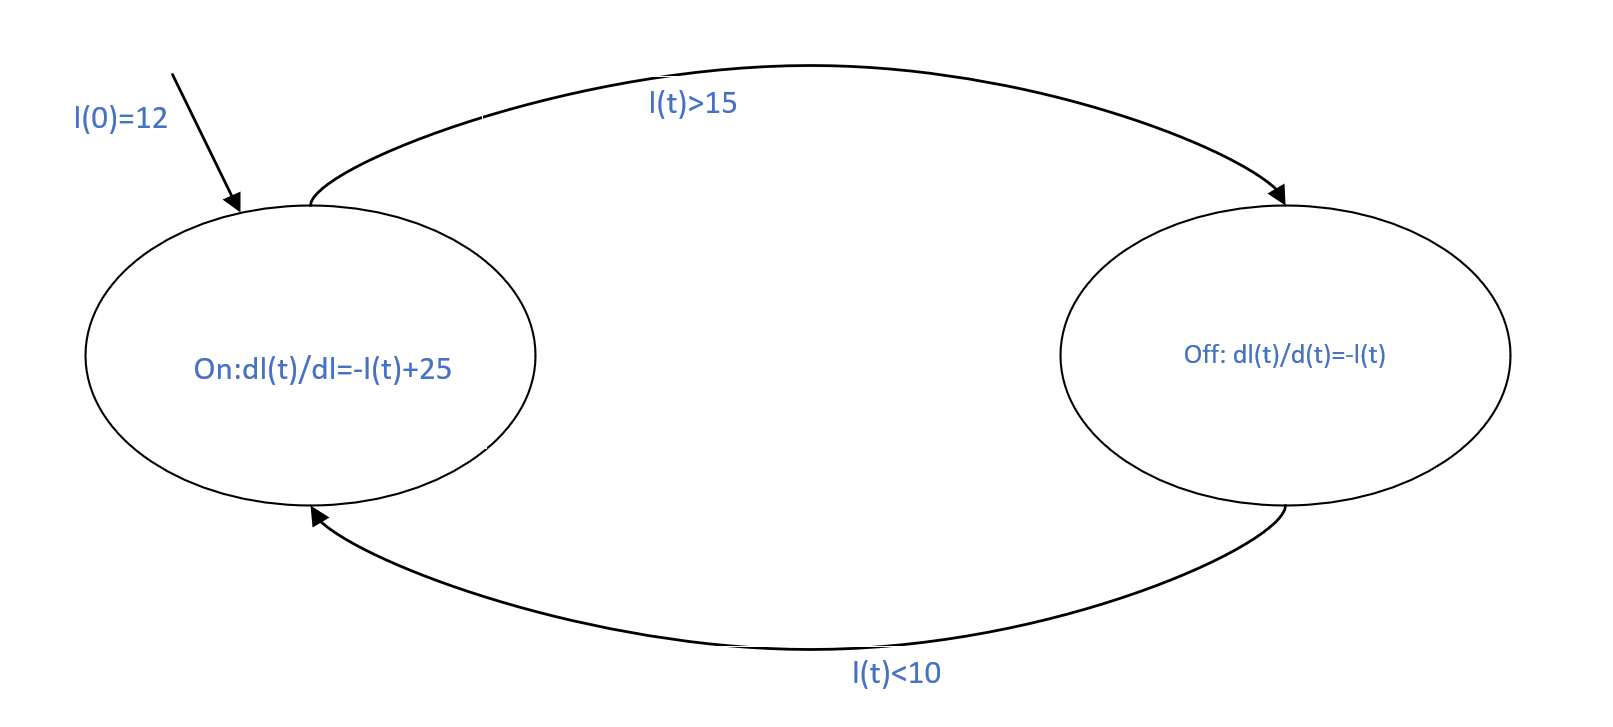
\includegraphics[width=0.9\textwidth]{images/automataa.png}
 \caption{Automata}
 \label{a}
\end{figure}

\subsection{b}

I used Simulink to do this modeling:
\begin{figure}[H]
 \centering
 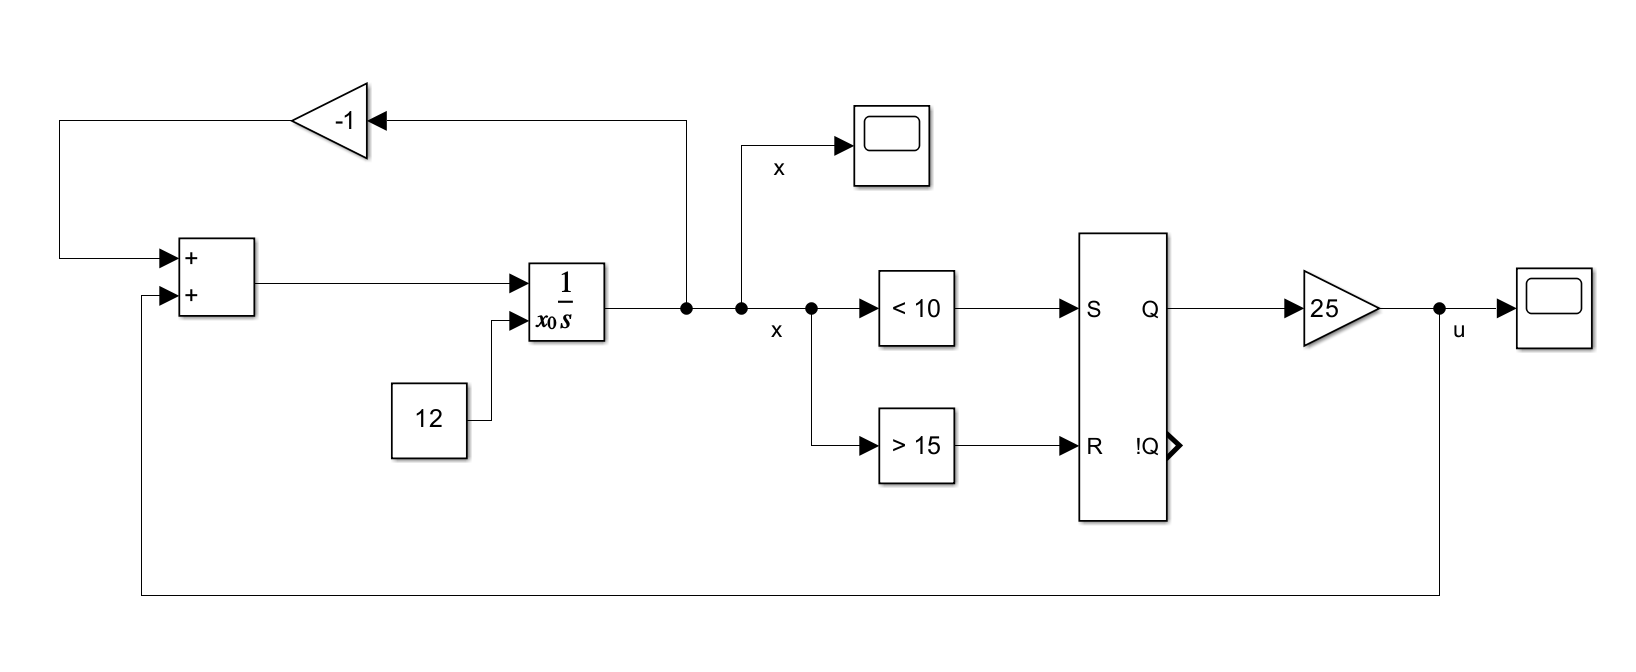
\includegraphics[width=0.9\textwidth]{images/model.png}
 \caption{Model in Simulink}
 \label{model}
\end{figure}

Here in figure \ref{compare-zero-crossing} shows the difference between with and without zero-crossing detection enabled with variable step solver.

\begin{figure}[h]
    \centering
    \begin{subfigure}[b]{0.9\textwidth}
        \centering
        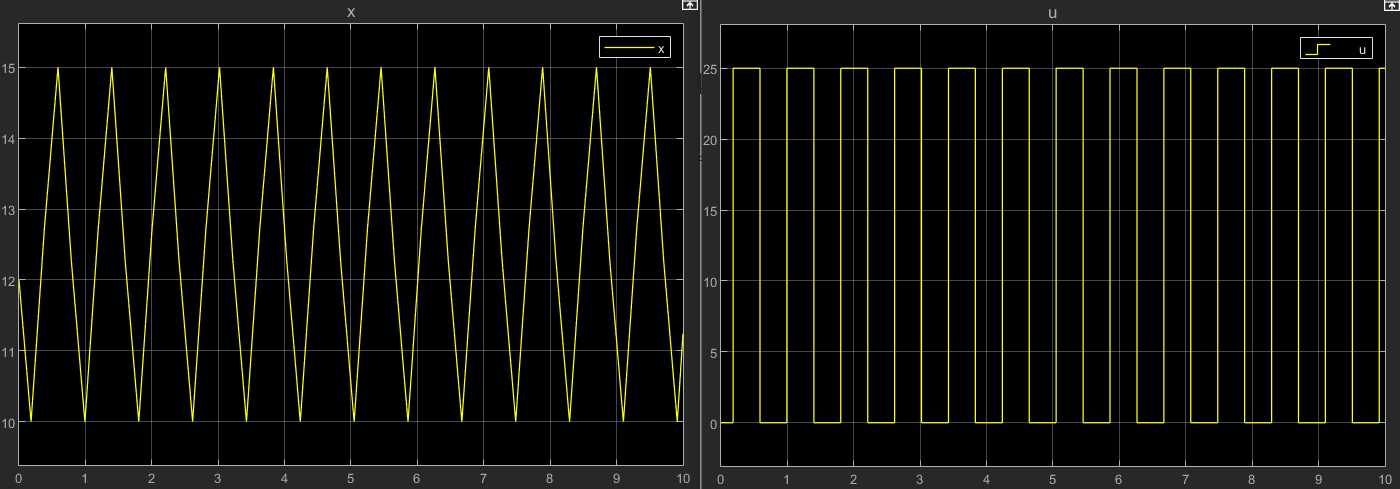
\includegraphics[width=\textwidth]{images/withzerocrossing.png}
        \caption{With Zero Crossing}
        \label{with}
    \end{subfigure}
    \hfill
    \begin{subfigure}[b]{0.9\textwidth}
        \centering
        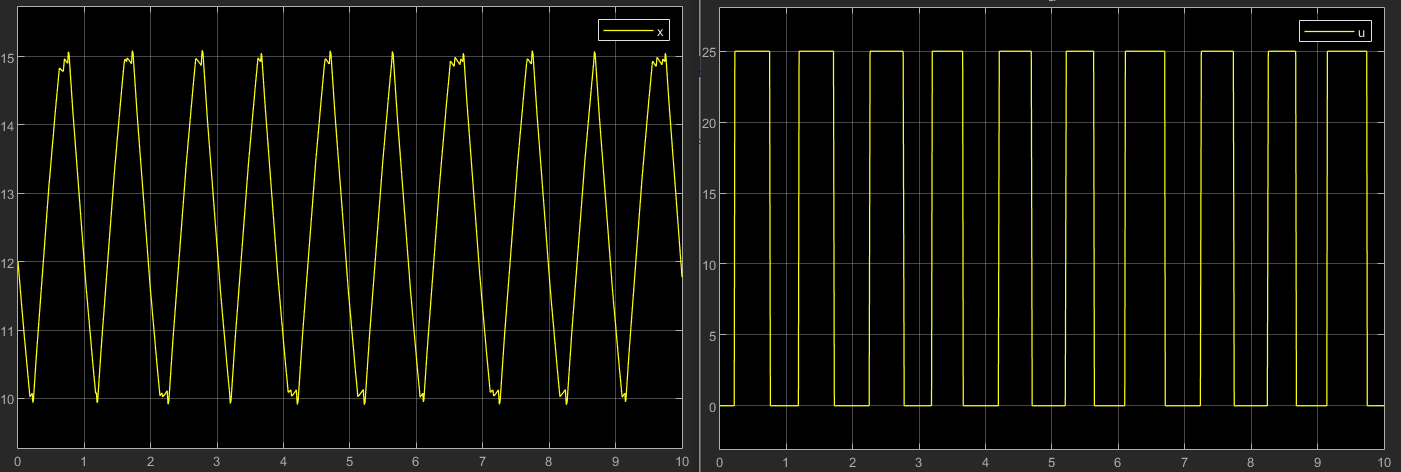
\includegraphics[width=\textwidth]{images/withoutzerocrossing.png}
        \caption{Without Zero Crossing}
        \label{without}
    \end{subfigure}
    \caption{Comparison of Zero Crossing on/off for variable step}
    \label{compare-zero-crossing}
\end{figure}

As you can see, there is a 'shake' on the peak, but it is not easy to analyze and it can not match the lecture.

Now to change the solver to Fixstep:

\begin{figure}[h]
    \centering
    \begin{minipage}{.5\textwidth}
      \centering
      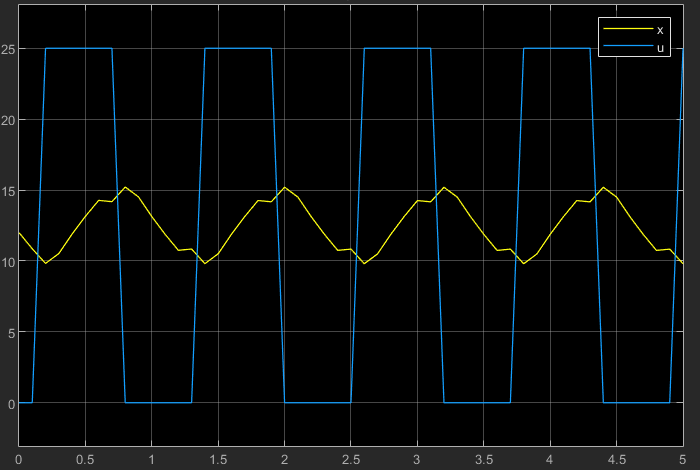
\includegraphics[width=0.8\linewidth]{images/disableall.png}
      \caption{Off}
      \label{disableall}
    \end{minipage}%
    \begin{minipage}{.5\textwidth}
      \centering
      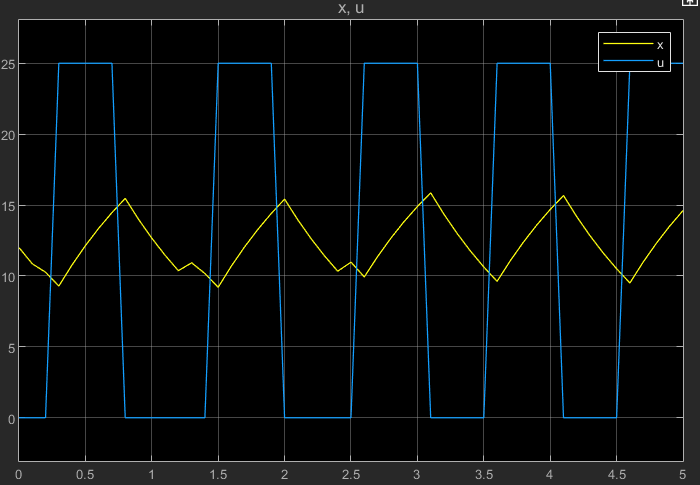
\includegraphics[width=0.8\linewidth]{images/enabledall.png}
      \caption{On}
      \label{enabledall}
    \end{minipage}
    \caption{Comparison of Off and On in Fixstep}
    \label{offandon}
    \end{figure}

    We can see it is obvious with the zero-crossing option enabled the state curve becomes smooth at the edge of the control signal u.

\subsection{c}

Zeno behavior occurs when the system appears to repeatedly approach a limit or event horizon without actually reaching it, but in our system, there is a gap between two event horizons so the Zeno behavior cannot approach.
%%%%%%%%%%%%%%%%%%%%%%%%%%%%%%%%%%%%%%%%%%%%%%%%%%%%%%%%%%%%%
\end{document}
